\documentclass{IEEEtran}%[conference]{IEEEtran}%\documentclass[10pt]{article}%{article}{report}{letter}{book}{proc}{slides}%
\usepackage{amsmath}
\usepackage{amssymb}
\usepackage{amsthm}
\usepackage{hyperref}
\usepackage{graphicx}
\usepackage{wasysym}
\usepackage{skull}

\hypersetup{colorlinks=true,linkcolor=blue,citecolor=blue}

%\textwidth=5.5in
%\oddsidemargin=0.5in
%\evensidemargin=0.0in
%\textheight=8.0in
%\topmargin=0.0in



\begin{document}

\title{Delay Comparison of Different Switch Architectures}



% author names and affiliations
% use a multiple column layout for up to three different
% affiliations
%\author{Stephan Adams and Libin Jiang}
%\IEEEauthorblockA{Department of Electrical Engineering and Computer Science\\
%University of California, Berkeley\\
%\{shadams, jnchang\}@eecs.berkeley.edu}
\author{\IEEEauthorblockN{S. H. Adams, L. Huang, A. Parekh, and J. Walrand \\}}
%\IEEEauthorblockA{Department of Electrical Engineering and Computer Science\\
%University of California, Berkeley\\
%\{shadams,jnchang\}@eecs.berkeley.edu}}


% conference papers do not typically use \thanks and this command
% is locked out in conference mode. If really needed, such as for
% the acknowledgment of grants, issue a \IEEEoverridecommandlockouts
% after \documentclass

% use for special paper notices
%\IEEEspecialpapernotice{(Invited Paper)}

% make the title area


\maketitle

{\abstract
 We compare Iterative Slip (CITE MCKEOWN) and QCSMA (CITE LIBIN), find that considering packet size difference is very important to take into consideration.
\begin{itemize}
\item Metric is Delay (makes sense in DataCenter Environments)
\item Delay VS Throughput result changes dramatically depending on packet size assumptions
\item TCP acts as expected
\end{itemize}
}

\section{Introduction}
Computer networks have made their way to the core of our modern lifestyles.  Almost any information can (and often must) be found on the internet.  Many of the services people use on a daily basis rely on distributed processing of requests housed in enormous datacenters scattered across the country and the world.  All these networks require good routing technologies to be possible.

What is the best way to measure the efficacy of a router?  Two ways that come to mind are throughput and delay characteristics of the switches.  Traditionally routers have been evaluated based on their throughput performance.  This is an excellent metric as in the heart of the internet routing paths are subject to too much uncertainty to hope that optimizing the delays to carry over to the roundtrip time of your packets.

On the other hand, in a datacenter setting the paths are no longer uncertain, as the whole network is controlled by a single entity, so delay again becomes a metric that is worth considering.  The other reason that delay optimization (on top of throughput) is a good idea is that the distributed nature of the applications run on datacenters is often very delay sensitive.  For instance in a google data center any search query must be returned within 300 milliseconds? (CITE SOMEONE) or the work done must be discarded.

Although delay is clearly a very important metric to consider in these settings, it is not as readily analyzed as throughput, which makes it more difficult to give a reliable a design recommendation.  In order to model the effects of different switch schedulers we have built a network simulator using assumptions meant to mimic a datacenter environment.  We have compared the performance of two relevant scheduling architectures in the hopes of demonstrating that provable throughput optimality can lead to an improvement in delay performance when switches are subjected to high loads.

\begin{itemize}
\item Routers are a core piece of our networks
\item Need simple scheduling policies, since volume of traffic strongly penalizes per packet overheads 
\item In the internet throughput is right metric -- can't make up for other delays in network
\item In Data centers have enough control over other switches that delay becomes a good metric.
\item Evolution of Routers -- SLIP killed head of Line delays but can't really be analyzed
\item QCSMA -- solves NP hard problem, but may cause large delays?
\item Question:  Should the optimality of QCSMA not show up in some performance gains over slip?  (In particular wrt delay?)
\end{itemize}


\section{Schedulers}
\begin{itemize}
\item How they work
\item Design Philosophy
\item Expected Properties
\end{itemize}
\section{Switch Schedulers}
We consider two different scheduling algorithms used to route packets across a crossbar based switch.  Iterative Slip -- a practical scheme design by Nick McKeown to solve the issues of head of line delay \cite{McKeown}, and QCSMA -- a probabilistic scheduling policy developed and optimized to be full throughput by Libin Jiang \cite{Libin}.

The assumption about the hardware for both our switches is the same, the only differentiating component is the scheduler which determines which set of packets will be transmitted at each transmission opportunity.  A good scheduler can support an arbitrarily high load, and provides a low delay per packet.  In practice the scheduler will incur some overhead because it takes time to generate a feasible transmission schedule.  The schedulers we use an (ideally) small number of contention slots at the beginning of each packet transmission opportunity during which the inputs and the outputs can exchange information to determine the best schedule.  The communication mechanism between the inputs and outputs can be quite powerful in practice.  We assume that each input is connected to each output by a bidirectional one bit line. This allows each output and input to exchange 1 bit in each contention slot.  For the Slip based scheduler the packets are broken into smaller cells so that the schedules can be generated for a given set of cells, after which they are transmitted over the crossbar, and then the process is repeated.  The QCSMA based algorithms do not synchronize scheduling times, rather it is constantly generating new schedules across the unused portion of the crossbar.

\subsection{SLIP}

SLIP is a very intuitive and practical scheme invented by Nick Mckeown \cite{McKeown}.  It has been implemented in real systems and yields extremely good performance.  It is difficult to prove anything about this scheduler, but simulations show that it performs very well in many key loading regimes.\\

{\it How it works:}

The motivation behind SLIP was to develop a simple protocol that avoids the use of randomization in the scheduler.  SLIP achieves this by adding a very simple state to the switch.  Each input keeps track of the output to which it last transmitted a packet.  Similarly each output keeps track of the last input from which it received a packet.  Armed with this information,the switch follows these three phases in each contention slot:\\

{\bf SLIP Phases}
\begin{itemize}
\item 1) Every {\it unscheduled} input sends requests to the outputs for which it has at least one packet to deliver.
\item 2) Every {\it unscheduled} output admits the packet request from the input giving round robin priority from the last input it served ($s'$). i.e. first admitting requests from $s'+1$ then $s'+2$ etc.
\item 3) Every input schedules itself for the output that admitted it giving a round robin priority from the last output it transmitted through ($d'$).  i.e. first scheduling an admission from $d'+1$ then $d'+2$ etc.\\
\end{itemize}

After all the last contention slot the scheduled input and outputs transmit a single packet and update their state, after which the cycle continues.  Note that since the time it takes to transmit a packet depends on its length, there will be a lot of idle time in the system if packet length varies significantly.  In practice this is addressed by breaking packets up into small equal sized cells so scheduling can be done on a cell by cell basis as opposed to a packet by packet basis.  In our simulations we consider both the case of all packets being the same size, and the case in which there is a bimodal distribution of packet sizes.  The overhead necessary to split packets into smaller cells involves adding a header to each cell, and using a larger number of contention slots since they will be needed to schedule per cell size, not packet size.  In our simulations we assumed both of these contributed only a negligible amount to the total delay.

\subsection{Ideal QCSMA}

%Throughput optimal  --> Invented/Explored by Libin and Jean? --> Difficult to Implement

QCSMA is a throughput optimal scheme inspired by Carrier Sense Multiple Access protocols developed for scheduling nodes in a wireless environment.  Because it was designed for wireless environments it assumes a much more restricted feedback model than that used by SLIP, which may be one of the reasons that the practical implementations perform worse than expected.  The only feedback traditional QCSMA assumes to be available takes the form of a broadcast to all inputs or outputs. This differs markedly from the crossbar where it is possible to provide individual feedback to each input and outputs.%, which we will revisit later.

Still ideal QCSMA, is guaranteed to be full throughput.  Unfortunately the delay performance of priority flows will depend on the backlog of the queues which they enter, which penalizes low rate flows.  The ideal QCSMA takes place in continuous time and so is not constrained by the number of contention slots allotted to the scheduler, and thus represents a performance bound for the other schedulers.\\

{\it How it works:}

At the beginning of each transmission opportunity, each input $s$ generates an exponential timer $X_{s,d}$ for each nonempty queue  destined for output $d$ (denoted as $Q_{s,d}$).  $X_{s,d}$ is distributed with rate $\lambda_{s,d} = (Q_{s,d})^{\alpha}$.  Where $\alpha > 0$ is a parameter to be chosen.  Input $s$ then requests access to output $d$ when timer $X_{s,d}$ expires. \\ %There will be no collisions  as this happens in continuous time.\\

{\bf Ideal QCSMA:}
\begin{itemize}
\item {\it unscheduled} input queue $Q_{s,d}$ generates timer value $X_{s,d}\sim \text{exp}(Q_{s,d}^\alpha)$
\item When $X_{s,d}$ expires schedule transmission from input $s$ to output $d$ unless $d$ or $s$ is already scheduled.
\item When all timers expire transmit packets.\\
\end{itemize}

Note the probability of a collision (two or more inputs requesting access to the same output simultaneously) is 0 when the timer values $X_{s,d}$ are continuous.  In simulations we assume that the timer resolution period takes no time, so this scheduling policy can act as an idealized performance benchmark.  This is impossible to implement, so it is necessary to develop a time slotted version that works in a finite number of discrete of contention slots.  Because we assume uniform packet sizes, and synchronized scheduling, all inputs compete for all outputs at the beginning of each transmission opportunity.  This may negatively impact observed performance.% although this is unimplementable.  Also note that QCSMA is inspired by Carrier Sense Multiple Access protocols which do not take advantage of the more fine grained feedback available in the switch context, and leveraged by SLIP.

\subsection{Slotted QCSMA} \label{naive_qcsma}

%Approximation of Ideal QCSMA  -->  Hope for similar performance -- Needed to be tweaked to 

In a real system it is not possible to implement continuous time counters, so it is necessary to approximate the continuous time scheduler with a discrete time system.  The scheduling requests for a given output from a given source are made whenever both that output and source are not transmitting any packets and so is not limited to a fixed number of contention slots like that of Slip.  (We can think of it as in every time slot, performing QCSMA on the portion of the crossbar that is idle.)  Slotted QCSMA approximated exponential timers by geometric random variables determining in which time slot the transmission requests should be made.

If each time slot is assumed to have duration $\beta$, then the probability that an exponential timer of rate $Q_{s,d}^\alpha$ expires within a time slot is given by:
\begin{align}
p'_{s,d} =1-e^{\beta Q_{s,d}^\alpha} \approx \beta Q_{s,d}^\alpha
\end{align}
% in  geometric random variable used to approximate the exponential can approximated by:
If we take $p'_{s,d}$ to be the request probability of the input $s$ to output $d$.  When queues get arbitrarily large, the collisions in the system may get excessively large (and therefore block transmissions indefinitely), so we limit the aggressiveness of the request rate in order to limit the number of collisions by defining:
\begin{align}  \label{geo_p}
p_{s,d} =\min \left[ \beta Q_{s,d}^\alpha,p_{\text{cap}}\right]
\end{align}

Where we chose $p_{\text{cap}}=.2$.  This then yields the following practical scheme:\\

{\bf Slotted QCSMA:}
\begin{itemize}
\item In the first contention slot for the packet transmission opportunity each input queue calculates $p_{s,d}$
\item {\it unscheduled} input queue $Q_{s,d}$ requests output $d$ with probability $p_{s,d}$.
\item Output $d$ announces the outcome of requests to it.  If there is only one request, $d$ reports success.  Upon multiple requests, $d$ reports collision. For no requests, $d$ reports no transmission.
\item If the requests of input $s$ were successful to the outputs in the set $\mathcal{D}$, $s$ schedules itself to output $d$ with probability $\frac{Q_{s,d}}{\sum_{d\in \mathcal{D}}Q_{s,d}}$ (i.e. $s$ chooses among its transmission opportunities in proportion to the queue lengths)
\item Unsuccessful inputs update $p_{s,d}$ according to one of the schemes below, and re start requesting process\\
\end{itemize}

The performance of this algorithm is expected be quite bad when the packets all have the same length, as it will yield a large number of queues competing for an output at the same time, and therefore also an increased chance of collision.  One possible approach to mitigate this is to adjust the request probabilities using an adaptive sheme. such as the one first proposed by Hajek and van Loon \cite{Hajek_van_Loon}, which was proven to be optimal in wireless environments.  The base probabilities are multiplied by $(1.518,1.000,.559)$  in the event of (no transmission, success, collision).  While this does require a trinary broadcast at the end of each contention slot it is possible to implement the feedback with a binary broadcast as well.  We have shied away from this approach, to compare just the simplest case performance of our different algorithms.

\section{Experiments}
\begin{itemize}
\item Uniform Packet Sizes VS More Realistic Setting
\item Parameter Choices
\item Load Graphs
\item TCP Graphs Choice of Load Patterns
\end{itemize}

\section{Simulator}

To compare the delay performance of the different schedulers we built an event driven simulators in C++.  All the graphs were plotted for $32 \times 32$ switches (i.e. 32 inputs and 32 outputs).  Simulation time is discrete with the minimum time step assumed to be the length of one of the bit transmissions of one of the schedulers.   The packet lengths are given in lengths of these time steps.  Because modern crossbars are transmit packets in parallel we assume that it takes 5 clock ticks to transmit a 64 byte packet, and 120 clock ticks to transmit a 1500 byte packet.  For all the Slip simulations we assumed there were $6$ contention slots used to generate the crossbar schedules, but that these calculations were pipelined in such a way as to make the net scheduling was negligible compared to the packet transmission time.  Simulation inputs were flow patterns passing through the switch, which were identical for all switches. %The switch operation was simulated for $10^6$ time steps, in order to reach the steady state switch behavior%during a given experiment in order to avoid  make the comparison between different scheduling policies and module types without worrying about inconsistencies in flow statistics.   

 The simulations fell into two categories: an open loop version meant to measure switch throughput, and a closed loop version meant to mimic TCP operation over the switch.  %We go into more depth in subsequent sections.
 
\section{Open Loop Simulations}

We explored the capacity of the different schedulers by injecting a stream of packets at a given rate into the switch.  For the QCSMA algorithms we also had to do a search for good parameters, and settled on the values in table \ref{qcsma_parameters}.  Once the appropriate parameters had been chosen we generated figures \ref{one_size} and \ref{variable_size} by performing multiple simulations by increasing the fraction $f$ of switch capacity from $.1$ to $.95$.  The load was generated by having flows from every input $s$ to every output $d$.  In each time step, each flow received a new packet with an i.i.d. probability $p=f/32$.

\begin{table}[ht] \caption{QCSMA Parameters} 
\centering 
\begin{tabular}{c c c}
 \hline\hline 
 Algorithm & $\beta$ & $\alpha$ \\
  [0.5ex] \hline 
   QCSMA&.2&.9  \\
   ideal  QCSMA&-&1  \\
   %DCSMA&?&?  \\
  [1ex] \hline 
  \end{tabular}
   \label{qcsma_parameters} 
\end{table}

In figure \ref{one_size}, all the packets were generated to have one size.  In this scenario Slip performs very well, on par with ideal QCSMA.  Slotted QCSMA incurs the largest delays.

In order to test whether this poor performance was due to the higher collision rate caused by all the packet transmissions beginning and ending almost simultaneously, we performed a second experiment in which we had a bimodal packet distribution over packet lengths.  In this alternate scenario (depicted in figure \ref{variable_size}) we generated packets with an iid probability of being the maximum size (1500 bytes) with probability $1/2$ and the minimum size (64 bytes) with probability $1/2$.  The rationale behind this distribution was to observe that data packets in TCP flows are generally transferring chunks of some larger file (so may as well send the maximum bytes).  For every data packet which makes it through the system, there is a control message, such as an ACK that do not need to be very large so can be modeled as being the minimum data packets.  As shown in figure \ref{variable_size} all the schedulers perform comparably until we reach higher loads.  Above loads of $60\%$ the switch capacity, Slip starts to perform considerably worse than slotted QCSMA.  Interestingly the performance of the slotted QCSMA follows the performance of the ideal version more closely than in the single packet length scenario.

\begin{figure}%[h]
	 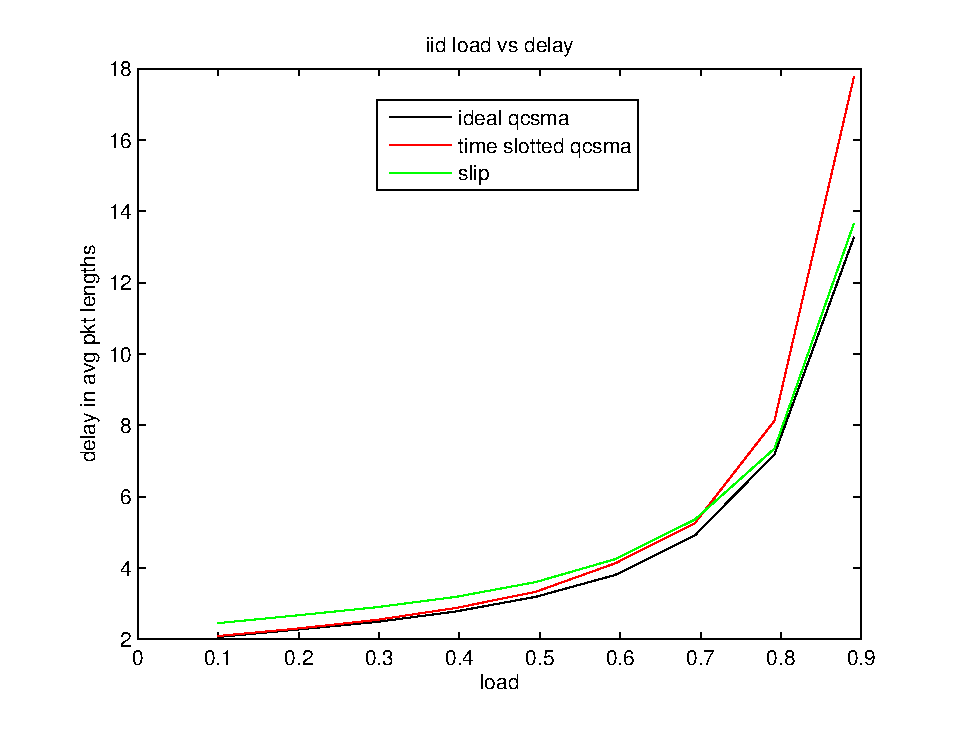
\includegraphics[width=90mm]{us_load.eps}
	\caption{Delay vs throughput graphs for loads in a scenario in which all packet have the same length.  Slip performs comparably to the ideal QCSMA scheduler, and outperforms the realistic implementation of QCSMA.  The parameters for the QCSMA based schedulers are taken from table \ref{qcsma_parameters}.} 	
	\label{one_size}
\end{figure}

\begin{figure}%[h]
	 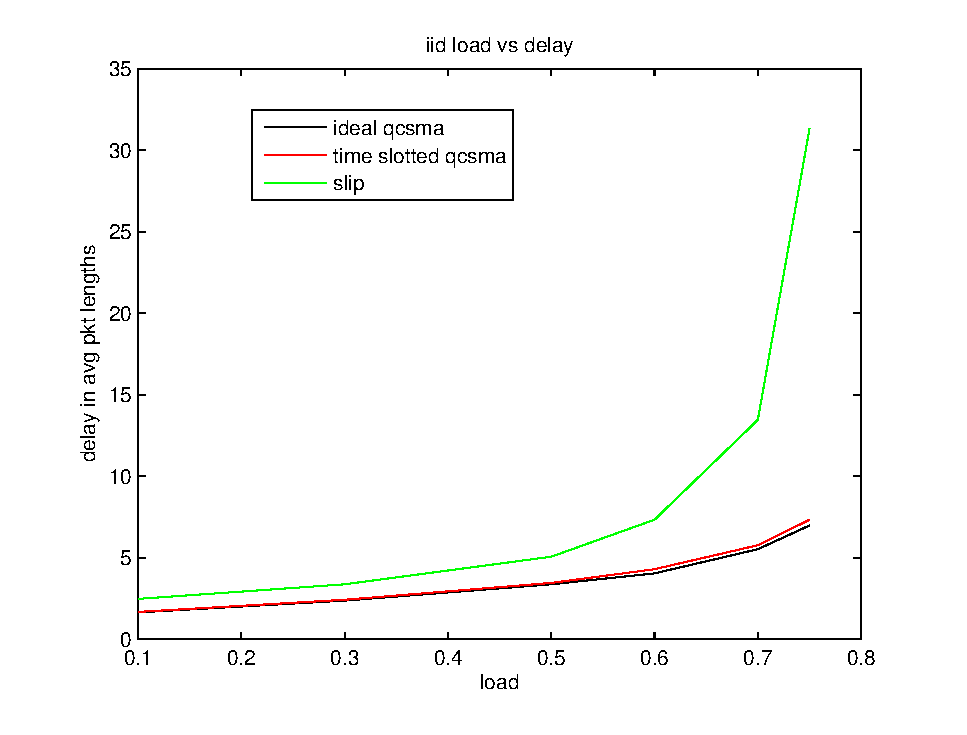
\includegraphics[width=90mm]{vs_load.eps}
	\caption{Delay vs throughput graphs for loads in a scenario in which every packet has a probability of $1/2$ of being the minimum size and $1/2$ of being the maximum size. With the variable sized packets Slip no longer outperforms the practical version of QCSMA.  QCSMA still performs similarly to the single length scenario.  (Note that the x axis in this graph is different from that in figure \ref{one_size}.) The parameters for the QCSMA based schedulers are taken from table \ref{qcsma_parameters}.} 	
	\label{variable_size}
\end{figure}

\section{Closed Loop (TCP) Simulations}
\begin{figure}%[h]
	% \includegraphics[width=90mm]{typical_flows.png}
	\caption{This graph represents the flow matrix of a `typical' datacenter load.  Where $80\%$ of the flows (type 2) generate a low volume of traffic and are sensitive to delays.  The other $20\%$ of flows (type 1) generate a large volume of traffic and are require a high throughput but not necessarily low delays.  The color in the $s,d$th position signifies the type of flow going from input $s$ to output $d$.  Flows of type $0$ do not generate any packets.} 	
	\label{typical_flows}
\end{figure}

Switches are not generally subjected to an unmodulated stream of packet flows.  Rather, the flows between applications are generally regulated via TCP or some other congestion/flow control mechanism.  This results in a different environment under which the differences highlighted by the open loop simulations might only play a negligible role.  To explore this idea, we have added a layer to our simulator which models TCP.  The only difference between our version of TCP and the traditional TCP is that we use Explicit Congestion Notification instead of packet dropping to respond to congestion.  Aside from simplifying the structure of the simulator, this choice reduces the long timeout delays, (or the need to fine tune the estimate of the roundtrip time to avoid this), which result whenever the routers buffers become overwhelmed.  The ECN bit is set with probability $p_{\text{ecn}}$ if the switch queues exceed some threshold $T_{\text{ecn}}$.  The TCP window is then reduced after it receives an ACK with the ECN bit set.  This is only one of the many proposed changes to adapt TCP to a datacenter setting.

We performed a variety of experiments meant to simulate different application communication patterns in datacenters.

As the throughput supported by the different switches seems comparable, we focus on the delay performance of the switches under TCP connections.  TCP Inputs to the simulator can be represented as a flow type matrix such as the one visualized in figure \ref{typical_flows}.  The entry $s,d$ represents the type of flow from input $s$ to output $d$.  We consider two main types of flows, high throughput flows that are relatively insensitive to delay (type 1 flows) and low throughput flows that are sensitive to delays (type 2 flows).  The packets generated for TCP transmission are generated according to Markov ON OFF processes much as in the open loop simulations with one producing a very low throughput set of packets and the other being generating a much higher throughput, in order to simulate the different types of datacenter flows.  The type 1 process has transitions from ON to OFF transition with probability $.3$ and from OFF to ON with probability $.7$.  The type 2 process transitions from ON to OFF with probability $0.0781$ and from OFF to ON with probability $0.9219$.  When the process is ON it generates packets, and it does not when it is OFF.   State transitions occur at each time step.

The TCP window size is updated by additive increase multiplicative decrease, with feedback coming in the form of acks that are generated whenever a packet successfully traverses the switch.  The acks in our simulation are not actually packets sent through our network, but rather simply notify our TCP simulator after an artificially determined delay.  After an ack notifies the TCP flow it adjusts its send window statistics accordingly.  The ack is delayed by a factor of 10 times the delay it took the packet to traverse the switch in order to simulate the round trip time in a datacenter that has five switches between the input and its intended output.\\


\subsubsection{Parameter Search}

In our model there is no maximum buffer size, and consequently no dropped packets.  Consequently, we need to give TCP feedback on when to halve its window size by another means.  We do this by using the explicit congestion control bit in the tcp header.  Our simulations mark packets as facing congestion with a probability $p_{\text{ecn}}$ if the packets arrive at a queue at or exceeding a threshold $T_{\text{ecn}}$ packets.  After our TCP receives an ack which announces that it faced congestion, it will halve it's window, and wait one round trip time before rehalving it's window, in order to flush out all the duplicate congestion announcements due to packets sent before the congestion announcement was received.


  TCP should be optimized for its environment so we conducted a parameter search to determine good values for each of the switches.  While the QCSMA was tuned to perform well for a worst case scenario, for TCP we are interested in improving average performance.  The search for the two parameters $p_{\text{ecn}}$ and $T_{\text{ecn}}$ is conducted over what we consider an average set of average flow statistics for a datacenter, as suggested in \cite{Benson} and \cite{Kandula} and shown in figure \ref{typical_flows}.

%As we assume the new datacenters will be built with a single scheduler in mind, so we search for good TCP parameters for each switch alternative.  
Please see table \ref{ecn_table} for the choices we settled on.  Once we settled on the parameters for TCP we can compare how the different architectures compare with each other for a variety of trial flows.  
%See the figures \ref{tcp_perf}.


We present 4 simulations in which we simulated different flow patterns to our schedulers and observed the average delay per flow.  The flow patterns we investigated were:

\begin{itemize}
\item all to all 
\item spread and aggregate 
%\item three simultaneous spread and aggregate
\item typical 
\item typical and spread and aggregate \\
\end{itemize}

\subsubsection{All to all (core switch)}
An all to all pattern can be seen in figure \ref{all_to_all}.  The type of each flow (from $s$ to $d$) was drawn from an iid distribution that yielded type 1 with probability $1/2$ and type 2 with probability $1/2$.  This flow pattern was meant to mimic a possible load on a core switch, which has to aggregate the traffic from across the network.  Results suggest that the performance of the switches was very similar.  The throughput for all the switches is about the same, and in terms of delay the difference is not significant. Ideal QCSMA performs mildly better than the other switches.  See figure \ref{all_to_all_delay} for a comparison.

Notably the gain of the unimplementable ideal QCSMA is negligible compared to that of SLIP, which does not have the same strong performance guarantees on throughput.  This will be a recurring theme in our findings.  Our implementation of a practical QCSMA, is comparable to SLIP but does perform slightly worse than SLIP.

\begin{figure}%[h]
	% \includegraphics[width=90mm]{all_to_all.png}
	\caption{This flow matrix is meant to model the traffic in a core switch.  Every input is connected to every output and the traffic carried is mixed between type 1 and type 2 flows.}
	\label{all_to_all}
\end{figure}

\begin{figure}%[h]
	% \includegraphics[width=90mm]{all_to_all_delay.eps}
	\caption{The per flow delay spread for the different schedulers under an all to all flow pattern.  Only the best 95\% of flows are shown to remove outliers.  The blue bar represents the spread between the best and worst flows and the red line represents the average value.  Clockwise from the top left we have timer simulating QCSMA, SLIP, and Ideal QCSMA.}
	\label{all_to_all_delay}
\end{figure}

\begin{table}[ht] \caption{TCP Parameters} 
\centering 
\begin{tabular}{c c c}
 \hline\hline 
 Switch & $T_{\text{ecn}}$ & $p_{\text{ecn}}$ \\
  [0.5ex] \hline 
  Benes&23&.5 \\
 SLIP&10&.5 \\
  QCSMA&12&.5  \\
   ideal  QCSMA&10&.9  \\
   %DCSMA&31&25  \\
  [1ex] \hline 
  \end{tabular}
   \label{ecn_table} 
\end{table}


\subsubsection{Spread and Aggregate (MapReduce)}
One of the most famous (if not most popular) applications in modern datacenters is certainly MapReduce.  The communication pattern of MapReduce often involves a large transfer of data to and from a single node between the different phases of computation.  In order to mimic this type of operation we developed a spread and aggregate flow pattern in which a given server sends data to all other servers using low throughput highly delay sensitive flows (type 2), which in turn are returned to the server.   An example in which the source of the pattern is on input 1 is shown in figure \ref{spreadagg}

This does not accurately model a MapReduce job for several reasons.  The biggest departure from a typical MapReduce job is that our type 2 flows do not have similar synchronization or burstiness properties due to the similar completion times of computations in a real MapReduce job.  Furthermore the large delays imposed by the artificial 10 hop distance for the acks is responsible for another difference in our model.  Still we hope that it suffices to give an impression of how a spread and aggregate application might behave.

The performance for the different crossbar applications is comparable as can be seen in figure \ref{spreadagg_delay_spread}.

\begin{figure}%[h]
	% \includegraphics[width=90mm]{spreadagg.png}
	\caption{This graph represents the flow matrix of a spread and aggregate pattern originating from input 1.  All flows are of type 2.}
	\label{spreadagg}
\end{figure}

\begin{figure}%[h]
%	 \includegraphics[width=90mm]{spreadagg_delay_spread.eps}
	\caption{This graph shows the delay spread of the flows under a simulated spread and aggregate pattern.}
	\label{spreadagg_delay_spread}
\end{figure}

\subsubsection{`Typical' datacenter flows}
The statistics in \cite{Benson} and \cite{Kandula} suggest that it is normal to have a relatively low utilization of the networks in modern datacenters.  In their findings they observed that only $10\%$ of the servers communicate.  They observed that $80\%$ of the flows had very short durations, while $20\%$ flows were really long lived and responsible for the majority of transmitted bits.  To model the bimodal behavior they observed we choose to use the two types of flows mentioned above.  A sample corresponding flow pattern for our simulations can be seen in figure \ref{typical_flows}.


In our simulations in this scenario all the crossbar based switches once again exhibited comparable performance (see figure \ref{typ_delays}).


\begin{figure}%[h]
	% \includegraphics[width=90mm]{typ_delays.eps}
	\caption{This graph represents the performance generated by a `typical' datacenter load with $80\%$ low throughput delay sensitive flows (type 2) and $20\%$ high throughput delay insensitive flows (type 1).}
	\label{typ_delays}
\end{figure}

\subsubsection{`Typical' Flows and spread and aggregate}
Finally to explore switch performance in a datacenter setting that supports both  `typical' datacenter loads and some MapReduce like jobs, we subjected the switch to a superposition of the datacenter load and two spread and aggregate loads on servers 1 and 11 as seen in figure \ref{typ_mult2}.  The performance of the crossbar based switches is again comparable (see figure \ref{typ_mult2_delays}), while the Benes switch exhibits significantly higher delays. The largest delays in the Benes switch taking more than three times as long as the worst crossbar design.

As can be seen in figure \ref{mixed_delay_matrix} the long delays are due to the spread and aggregate flows for all the switches, but for the Benes network they do especially badly.  Note that since it is the spread and aggregate flows (all type 2 flows) that suffer, figure \ref{typ_mult2_delays} shows type 2 as being particularly slow.  This is only true because the spread and aggregate flows are heavily delayed as opposed to the spread and aggregate flows slowing down other type 2 flows.  The other very interesting observation to make is that the incast flows in the Benes switch actually fair pretty well.  It is the many to one transmission that cannot take full advantage of the multipath and therefore incurs the large delays.
\begin{figure}%[h]
%	 \includegraphics[width=90mm]{mult2.png}
	\caption{This graph represents the mix of a `typical' load and two spread and aggregate jobs.}
	\label{typ_mult2}
\end{figure}

\begin{figure}%[h]
%	 \includegraphics[width=90mm]{mult2_flow_delays.eps}
	\caption{This graph represents the performance under a mix of spread and aggregate (on servers 1 and 11) and typical flows.}
	\label{typ_mult2_delays}
\end{figure}

\begin{figure}%[h]
%	 \includegraphics[width=90mm]{mult2_delay_matrix.png}
	\caption{This graph shows the average delay per flow for the mix of `typical' and spread and aggregate inputs.  The inputs originating the spread and aggregate flows (1 and 11) face the largest delays in the crossbar graphs, and here finally the ideal QCSMA differentiates itself from SLIP, but the practical QCSMA performance still remains comparable to SLIP.}
	\label{mixed_delay_matrix}
\end{figure}



\section{Conclusions}
\begin{itemize}
\item Differences in Packet Sizes Cannot be Neglected
\item QCSMA may perform better than slip when looking at delay optimization
\item TCP in datacenters...
\end{itemize}

\section{About Simulator:}
\begin{itemize}
\item Event Driven
\item variable collections
\item have state, events, and update functions
\item use memoryless thing
\item main loop
\item to change things need to change event merge, possibly the state, and which functions are called
\item event pictures
\end{itemize}

\section{Next Step:}
\begin{itemize}
\item pick suitable parameters
\item Build Experiments?
\end{itemize}
\section{To Do}
\begin{itemize}
\item Build Simulator: Now -- Oct 15th?
\item Perform Experiments: Oct 15th -- November 15th?
\item Write Paper: Now -- December 15th?
\item Time Line
\end{itemize}

\section{Simulator Pieces:}
\subsection{Crossbar}
\subsection{Scheduling Modules}
\subsection{Input Interface}
\subsection{Packet Generation}
\subsubsection{TCP Layer}
\subsubsection{Application Layer}
\subsection{Experiment Functions}
\subsection{Analysis Tools}
\subsubsection{Logs}
\subsubsection{Data Collection}
\subsubsection{Unit Tests}
\begin{itemize}
\item state is properly initialized
\item event merging
\item only real schedules are generated
\item right averages are attained
\item TCP waveforms are right when the channel is predictable
\item Event merge.
\end{itemize}
\subsubsection{Matlab Data Display Tools}
\subsection{Setting Parameters}


\section{Perform Experiments}

Try to mirror the experiments with the previous simulator as much as possible.
\subsection{What kind of packet distributions?}
Try bimodal distribution with high probability around a big size and small size with slight variations around the means.  Also single size with some slight variations.  Finally try without any of the small variations.
\subsection{What kind of Flow patterns?}
Start with those we have decided model the datacenter.
\subsection{Throughput Vs Delay Graphs}
\subsubsection{What are good parameters for QCSMA?}
\subsubsection{Number of Slots for SLIP}
\subsection{TCP performance}
\subsection{Performance Variation as packet sizes become more predictable}

\section{Write Paper}
\subsection{Would like to show: QCSMA is better than SLIP by x\%}
\subsection{Would like to show: Equal Length vs Variable Length Packets makes a big difference!}
\subsection{Simulator Documentation}
\subsubsection{Events and State}
\subsubsection{How to change things}

\label{bib}
\bibliography{MSThesis}{}
\bibliographystyle{plain} 
 
\end{document}